\documentclass[10pt,usenames,dvipsnames]{beamer}

\usepackage{amsmath}
\usepackage{stmaryrd}
\usepackage{centernot}
\usepackage{xspace}
\usepackage{listings}
\usepackage{hyperref}
\usepackage{xcolor}
\usepackage{graphicx}
\usepackage{macros}

%% Angelo's packages

\usepackage[utf8]{inputenx} % For æ, ø, å
\usepackage{csquotes}       % Quotation marks
\usepackage{microtype}      % Improved typography
\usepackage{amssymb}        % Mathematical symbols
\usepackage{mathtools}      % Mathematical symbols
\usepackage{stmaryrd}
\usepackage[absolute, overlay]{textpos} % Arbitrary placement
\setlength{\TPHorizModule}{\paperwidth} % Textpos units
\setlength{\TPVertModule}{\paperheight} % Textpos units
\usepackage{tikz}
\usetikzlibrary{overlay-beamer-styles}  % Overlay effects for TikZ
\usepackage{graphicx}
\usepackage{array}
\usepackage{amssymb}
\usepackage{stmaryrd}
\usepackage{subcaption}
\usepackage{float}
\usepackage{url}
\usepackage{doi}
\usepackage[all]{xy}

\lstset{language=Java,basicstyle=\ttfamily\footnotesize,commentstyle=\itshape,morekeywords={assert},keywordstyle=\ttfamily\bfseries}

%\usetheme[secfooter]{PaloAlto}
%\usetheme[secfooter]{Hannover}
%\usetheme[]{CambridgeUS}
\usetheme[secfooter]{UiB}

\usebackgroundtemplate{\hspace*{.85\textwidth}
\includegraphics[keepaspectratio,width=.2\textwidth]{images/logoBW.png}}

\title[Runtime Verification of Hash Code in Mutable Classes]{Runtime Verification of Hash Code in Mutable Classes} 

\author[D. Ancona]{\underline{Davide Ancona}, Angelo Ferrando and \\ Viviana Mascardi \\[1ex]
  \small DIBRIS, Universit\`a di Genova, Italy}

\institute[]{DIBRIS, Universit\`a di Genova, Italy}
\date[FTfJP23]{Formal Techniques for Java-like Languages, July 18, 2023}
\subject{}

%% \AtBeginSection[]
%% {
%%     \begin{frame}
%%         \frametitle{Table of Contents}
%%         \tableofcontents[currentsection]
%%     \end{frame}
%% }

\begin{document}

%%\frame{\titlepage}

\begin{frame}{Outline}
\tableofcontents%[currentsection]
\end{frame}

\section{Object equality and hash code}

\begin{frame}{Contract for equality and hash code}
  \begin{block}{Features of most object-oriented languages}
    \begin{itemize}
    \item two different notions of equality
      \begin{itemize}
      \item by reference, predefined (\lstinline{==})
      \item weaker equality, user-defined (\lstinline{equals})
      \end{itemize}
      \item hash code associated with an object
    \end{itemize}
  \end{block}

  \begin{block}{General contract in \lstinline[basicstyle=\ttfamily\large]{java.lang.Object}}
    \emph{If two objects are equal, then the same hash code must be computed for them}
  \end{block}

    \begin{block}{Reason}
      Classes as \lstinline{HashSet} or \lstinline{HashMap} rely on \lstinline{equals} and \lstinline{hashCode}:
      \begin{itemize}
      \item \lstinline{hashCode} is used to retrieve a specific bucket
      \item \lstinline{equals} is used to find an element in such a specific bucket        
        \end{itemize}
  \end{block}

\end{frame}

%%%%%%%%%%%%%%%%%%%%%%%%%%%%%%%%%%%%%%%%%%%%%%%%%%

\begin{frame}{Contract for equality and hash code}
  \begin{block}{A stricter contract in \lstinline{java.util.Set}}
    \emph{Great care must be exercised if mutable objects are used as set elements.}\\[1ex]
    \emph{The behavior of a set is not specified if the value of an object is changed in a way that affects equals comparisons while the object is an element in the set.} \\[1ex]
    \emph{A special case of this prohibition is that it is not permissible for a set to contain itself as an element.} 
  \end{block}
\end{frame}

%%%%%%%%%%%%%%%%%%%%%%%%%%%%%%%%%%%%%%%%%%%%%%%%%%

\begin{frame}[fragile]{Contract for equality and hash code}
  \begin{block}{A simple example}
    \begin{lstlisting}[language=Java]
var sset = new HashSet<Set<Integer>>();
var s = new HashSet<>(asList(1)); // s is {1}
sset.add(s); // sset is {{1}}
assert sset.contains(s); 
s.remove(1);
assert sset.contains(s); 
s.add(1);
assert sset.contains(s); 
    \end{lstlisting}
  \end{block}
\end{frame}

%%%%%%%%%%%%%%%%%%%%%%%%%%%%%%%%%%%%%%%%%%%%%%%%%%

\begin{frame}[fragile]{Contract for equality and hash code}
  \begin{block}{A simple example}
    \begin{lstlisting}[language=Java]
var sset = new HashSet<Set<Integer>>();
var s = new HashSet<>(asList(1)); // s is {1}
sset.add(s); // sset is {{1}}
assert sset.contains(s); // success
s.remove(1);
assert sset.contains(s); // failure
s.add(1);
assert sset.contains(s); // success
    \end{lstlisting}
  \end{block}
\end{frame}

%%%%%%%%%%%%%%%%%%%%%%%%%%%%%%%%%%%%%%%%%%%%%%%%%%

\begin{frame}[fragile]{Contract for equality and hash code}
  \begin{block}{Another example}
    \begin{lstlisting}[language=Java]
var sset = new HashSet<Set<Integer>>();
var s = new HashSet<>(asList(0)); // s is {0}
sset.add(s); // sset is {{0}}
assert sset.contains(s); 
s.remove(0);
assert sset.contains(s); 
s.add(0);
assert sset.contains(s); 
    \end{lstlisting}
  \end{block}
\end{frame}

%%%%%%%%%%%%%%%%%%%%%%%%%%%%%%%%%%%%%%%%%%%%%%%%%%

\begin{frame}[fragile]{Contract for equality and hash code}
  \begin{block}{Another example}
    \begin{lstlisting}[language=Java]
var sset = new HashSet<Set<Integer>>();
var s = new HashSet<>(asList(0)); // s is {0}
sset.add(s); // sset is {{0}}
assert sset.contains(s); // success
s.remove(0);
assert sset.contains(s); // success!
s.add(0);
assert sset.contains(s); // success
    \end{lstlisting}
  \end{block}

  \begin{block}{Issues}
    \begin{itemize}
    \item almost unpredictable code behavior
    \item non-deterministic behavior if \lstinline{hashCode} depends on object references
      \begin{itemize}
      \item object references may change from one execution to another 
      \item hash code needs not remain consistent from one execution to another 
      \end{itemize}    
    \end{itemize}    
  \end{block}
\end{frame}

%%%%%%%%%%%%%%%%%%%%%%%%%%%%%%%%%%%%%%%%%%%%%%%%%%

\begin{frame}[fragile]{Theory versus practice}
  \begin{block}{Theory}
    \begin{itemize}
    \item mutable classes should not redefine \lstinline{equals}
    \item weaker contract: \lstinline{hashCode} should not depend on ``mutable'' fields
    \end{itemize}   
  \end{block}

  \begin{block}{Practice}
    \begin{itemize}
    \item mutable classes of \lstinline{java.util.Collection} do not satisfy such a contract 
    \item similar problems in Kotlin and Scala, but not in C\#
    \end{itemize}   
  \end{block}


    \begin{block}{Aims}
    \begin{itemize}
    \item verify that \lstinline{Collection} objects are not modified while in a hash table
    \item proposed solution: Runtime Verification (RV)
    \item related work: study of \lstinline{equals} and \lstinline{hashCode} contract in Java collections
       [NelsonPearceNoble@TOOLS2010]
    \end{itemize}   
  \end{block}

\end{frame}

%%%%%%%%%%%%%%%%%%%%%%%%%%%%%%%%%%%%%%%%%%%%%%%%%%

\lstset{
	morekeywords={not,false,true,none,any,empty,matches,all,let,if,else,with,abs},
	keywordstyle=\color{blue},
	morestring=[b]',
	stringstyle=\color{violet},
	morecomment=[l]{//},
	commentstyle=\color{cyan},
	mathescape=true,
	basicstyle=\ttfamily,
	captionpos=b,
	tabsize=4,
	breaklines,
	breakatwhitespace,
	showstringspaces=false,
	keepspaces
}

\lstset{literate={\\/}{$\orop$}2 {/\\}{$\andop$}2 {|}{$\shuffleop$}1 {!}{$\closop$}1 {>>}{$\filterop$}2 {:}{$:$}1}

\section{Runtime Verification and \rml}

\begin{frame}{Runtime verification}

  \begin{block}{Definition}
    Runtime Verification (RV) is a \hl{verification technique} that allows for checking whether a \hl{run} of a system under scrutiny (SUS) \hl{satisfies or violates} a given correctness property.
  \end{block}

  \begin{block}{Main ingredients}
   \begin{itemize}
   \item run = possibly infinite event trace
   \item instrumentation = generates the relevant events
   \item formal specification = a set of event traces     
   \item monitor =  generated from a specification, dynamically checks finite prefixes of a run 
\end{itemize}
  \end{block}

\end{frame}

%%%%%%%%%%%%%%%%%%%%%%%%%%%%%%%%%%%%%%%%%%%%%%%%%%

\begin{frame}{Runtime verification}

  \begin{center}
    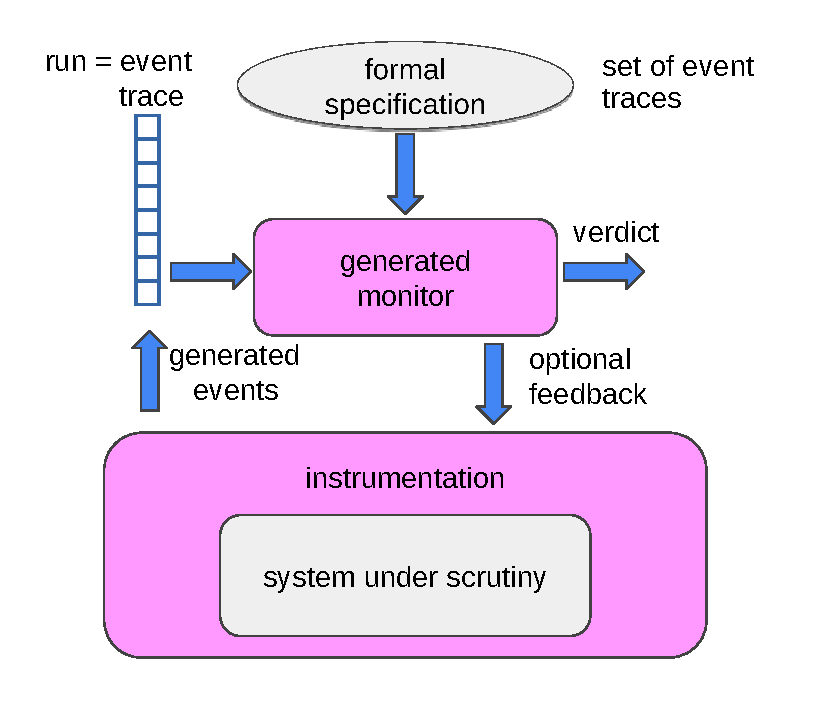
\includegraphics[keepaspectratio,height=0.7\textheight]{images/rv}
  \end{center}

\end{frame}

%%%%%%%%%%%%%%%%%%%%%%%%%%%%%%%%%%%%%%%%%%%%%%%%%%

\begin{frame}{Why RV?}
  \begin{block}{RV bridges the gap between formal verification and testing}
    \begin{itemize}
    \item as in formal verification
      \begin{itemize}
      \item properties defined with a formalism
      \item runs abstracted by event traces
      \end{itemize}
    \item as in testing
      \begin{itemize}
      \item scalable solution although non exhaustive
      \item exploitation of information available only at runtime
      \end{itemize}
    \item other features
      \begin{itemize}
      \item error recovery, self-adaptation, cast-iron guarantees
      \item runtime verification of control-oriented properties
      \end{itemize}
    \end{itemize}
  \end{block}
\end{frame}

%% \begin{frame}{RV taxonomy}
%%     \begin{figure}
%%         \centering
%%         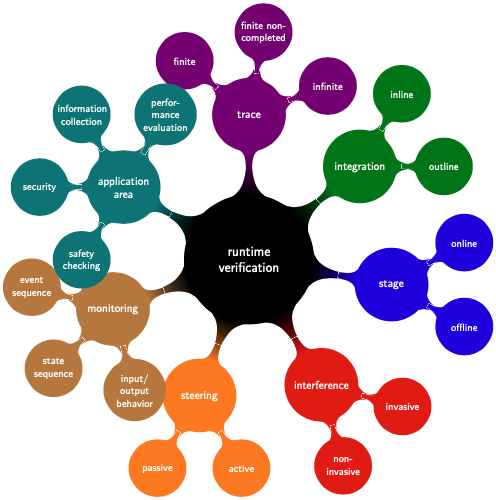
\includegraphics[width=0.59\linewidth]{images/example6.png}
%%     \end{figure}
%% \end{frame}

%% \begin{frame}{RV taxonomy}
%%   \begin{block}{Stages of monitoring}
%%     \begin{itemize}
%%     \item \hl{on line}
%%       \begin{itemize}
%%       \item during execution of the system
%%       \item storing of the trace unnecessary
%%       \item      supports runtime enforcement
%%       \end{itemize}
%%     \item \hl{off line}
%%       \begin{itemize}
%%       \item  after execution of the system, with the trace stored in log files
%%       \item      does not support runtime enforcement
%%       \item complementary to testing and debugging
%%       \end{itemize}
%%     \end{itemize}
%%   \end{block}

%% \end{frame}

%%%%%%%%%%%%%%%%%%%%%%%%%%%%%%%%%%%%%%%%%%%%%%%%%%

\begin{frame}{\rml}
  \begin{center}
    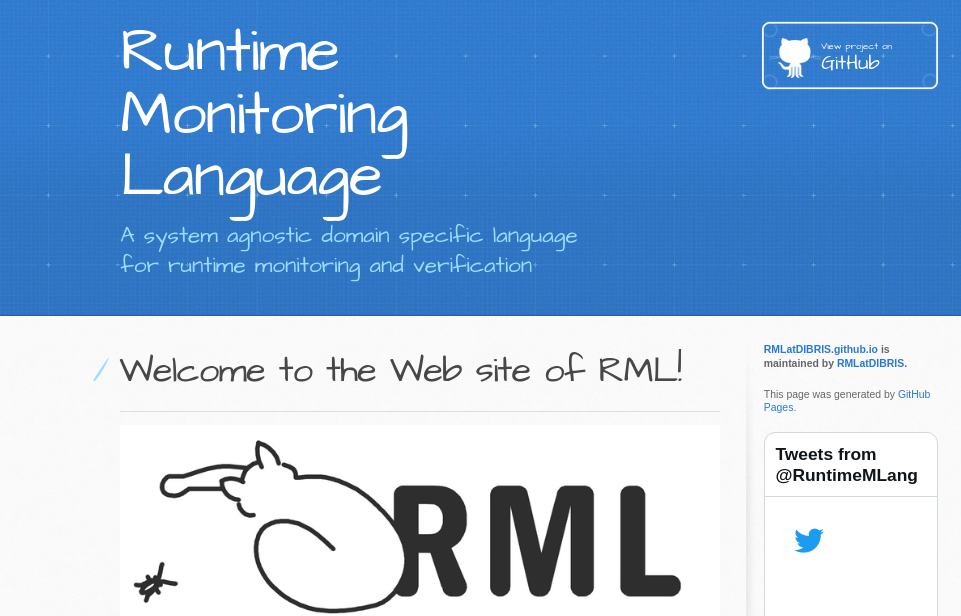
\includegraphics[height=0.7\textheight]{images/rmlweb}
  \end{center}

  \rml Web page: \href{https://rmlatdibris.github.io/}{https://rmlatdibris.github.io/}
\end{frame}

%%%%%%%%%%%%%%%%%%%%%%%%%%%%%%%%%%%%%%%%%%%%%%%%%%

\begin{frame}{\rml}

  \begin{block}{Main features of \rml}
    \begin{itemize}
    \item inspired by \hl{global session types}
    \item based on \hl{formal languages}: extension of deterministic CF grammars 
    \item \hl{usability}: developers are familiar with regular expressions and grammars
    \item \hl{expressive power}: more expressive than deterministic CF grammars
    \item \hl{interoperability}: separation between specification and instrumentation
    \end{itemize}
  \end{block}
\end{frame}

%%%%%%%%%%%%%%%%%%%%%%%%%%%%%%%%%%%%%%%%%%%%%%%%%%

\begin{frame}{Structure of \rml specifications}
  \begin{block}{Four layers}
    \begin{itemize}
    \item \hl{event types}: relevant events 
    \item \hl{trace expressions}: primitive and derived operators on sets of traces
    \item \hl{parametricity}: existential quantification w.r.t. data carried by events
    \item \hl{genericity}:  enhanced modularity, reuse and expressive power
    \end{itemize}
  \end{block}
\end{frame}

%%%%%%%%%%%%%%%%%%%%%%%%%%%%%%%%%%%%%%%%%%%%%%%%%%

\begin{frame}[fragile]{Events and event types in \rml}
  \begin{block}{An event trace}
    \begin{lstlisting}[basicstyle=\ttfamily\scriptsize]
$\ldots$
{"event":"func_pre","name":"add","targetId":5,"argIds":[13]}      
{"event":"func_post","name":"add","res":true,"targetId":5,"argIds":[13]}
{"event":"func_pre","name":"remove","targetId":5,"argIds":[9]}
{"event":"func_post","name":"remove","res":true,"targetId":5,"argIds":[9]}
$\ldots$
    \end{lstlisting}
  \end{block}

  \begin{block}{Event type declarations}
    \begin{lstlisting}[basicstyle=\ttfamily\scriptsize]
add(hash_id,elem_id) matches {event:'func_post', targetId:hash_id, name:'add', argIds:[elem_id], res:true};
remove(hash_id,elem_id) matches {event:'func_post', targetId:hash_id, name:'remove', argIds:[elem_id], res:true};

modify(targ_id) matches add(targ_id,_) | remove(targ_id,_);
    \end{lstlisting}
  \end{block}
\end{frame}

\begin{frame}[fragile]{\rml specifications}
  \begin{center}
    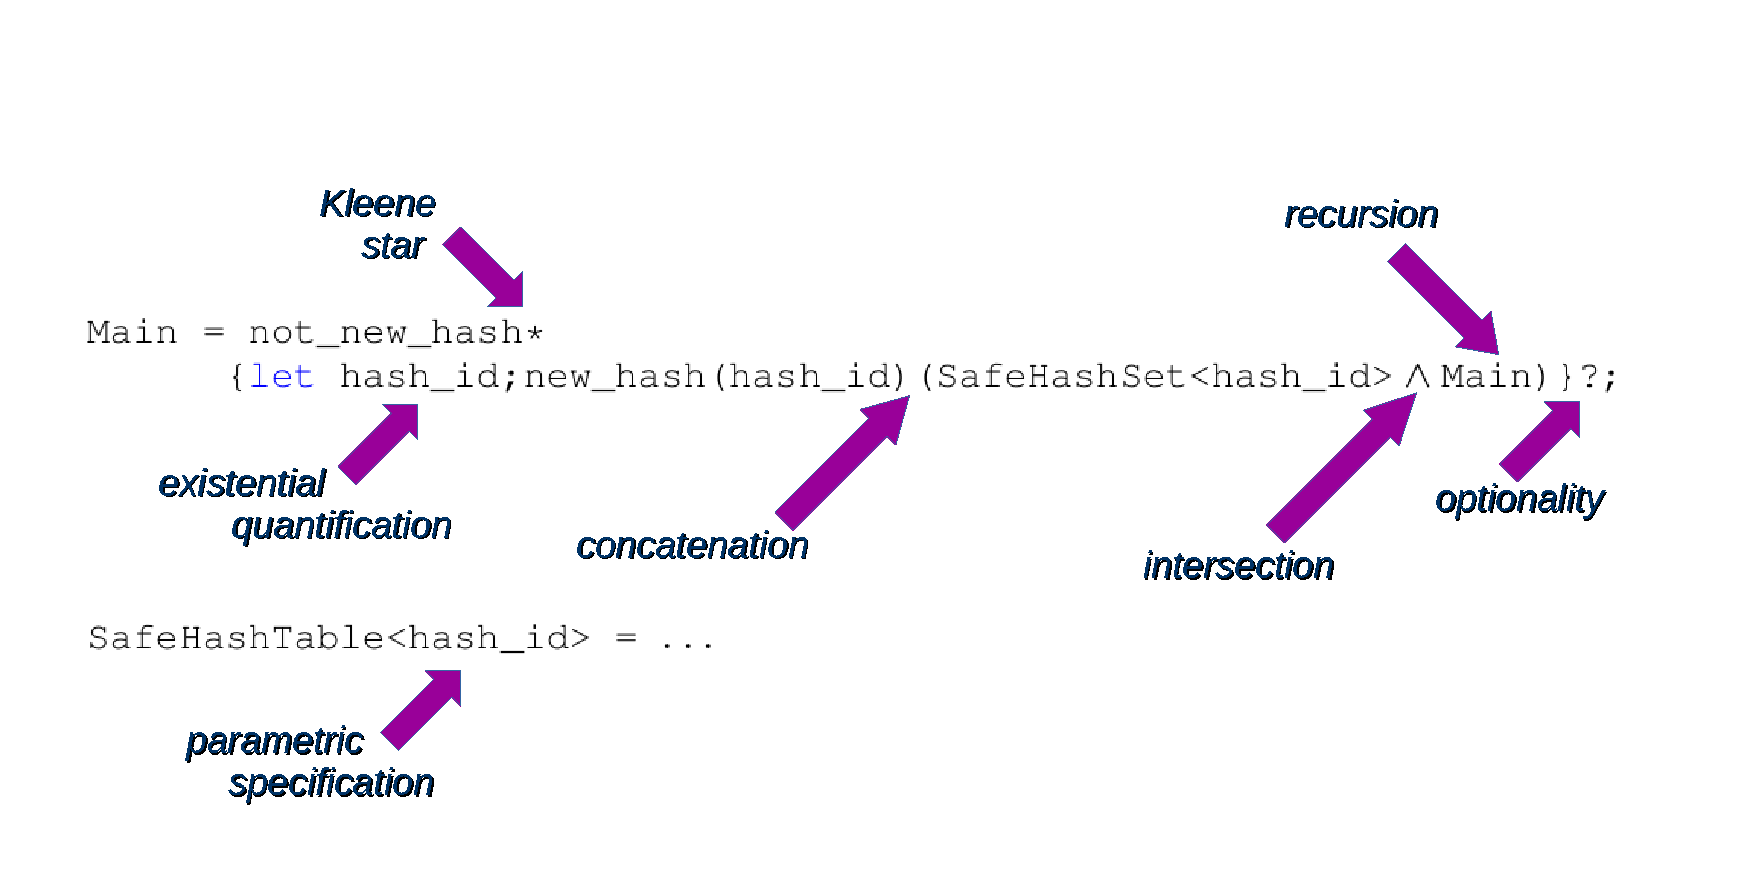
\includegraphics[keepaspectratio,width=1.4\textheight]{images/RMLfragAnnot2}
  \end{center}

%%        \begin{lstlisting}[basicstyle=\ttfamily\scriptsize]




%% Main = not_new_hash*
%%       {let hash_id;new_hash(hash_id)(SafeHashSet<hash_id>/\Main)}?;





%% SafeHashTable<hash_id> = $\ldots$
%%     \end{lstlisting}

\end{frame}

%%%%%%%%%%%%%%%%%%%%%%%%%%%%%%%%%%%%%%%%%%%%%%%%%%

\begin{frame}{\rml semantics}
  \begin{block}{In a nutshell}
    \begin{itemize}
    \item based on the notion of Brzozowski derivative 
    \item defined by a labeled transition systems with rewriting rules
    \item labels are the monitored events
    \item the initial state is the specification of the property
    \end{itemize}
  \end{block}
\end{frame}

%%%%%%%%%%%%%%%%%%%%%%%%%%%%%%%%%%%%%%%%%%%%%%%%%%

\begin{frame}{\rml semantics}
  \begin{center}
    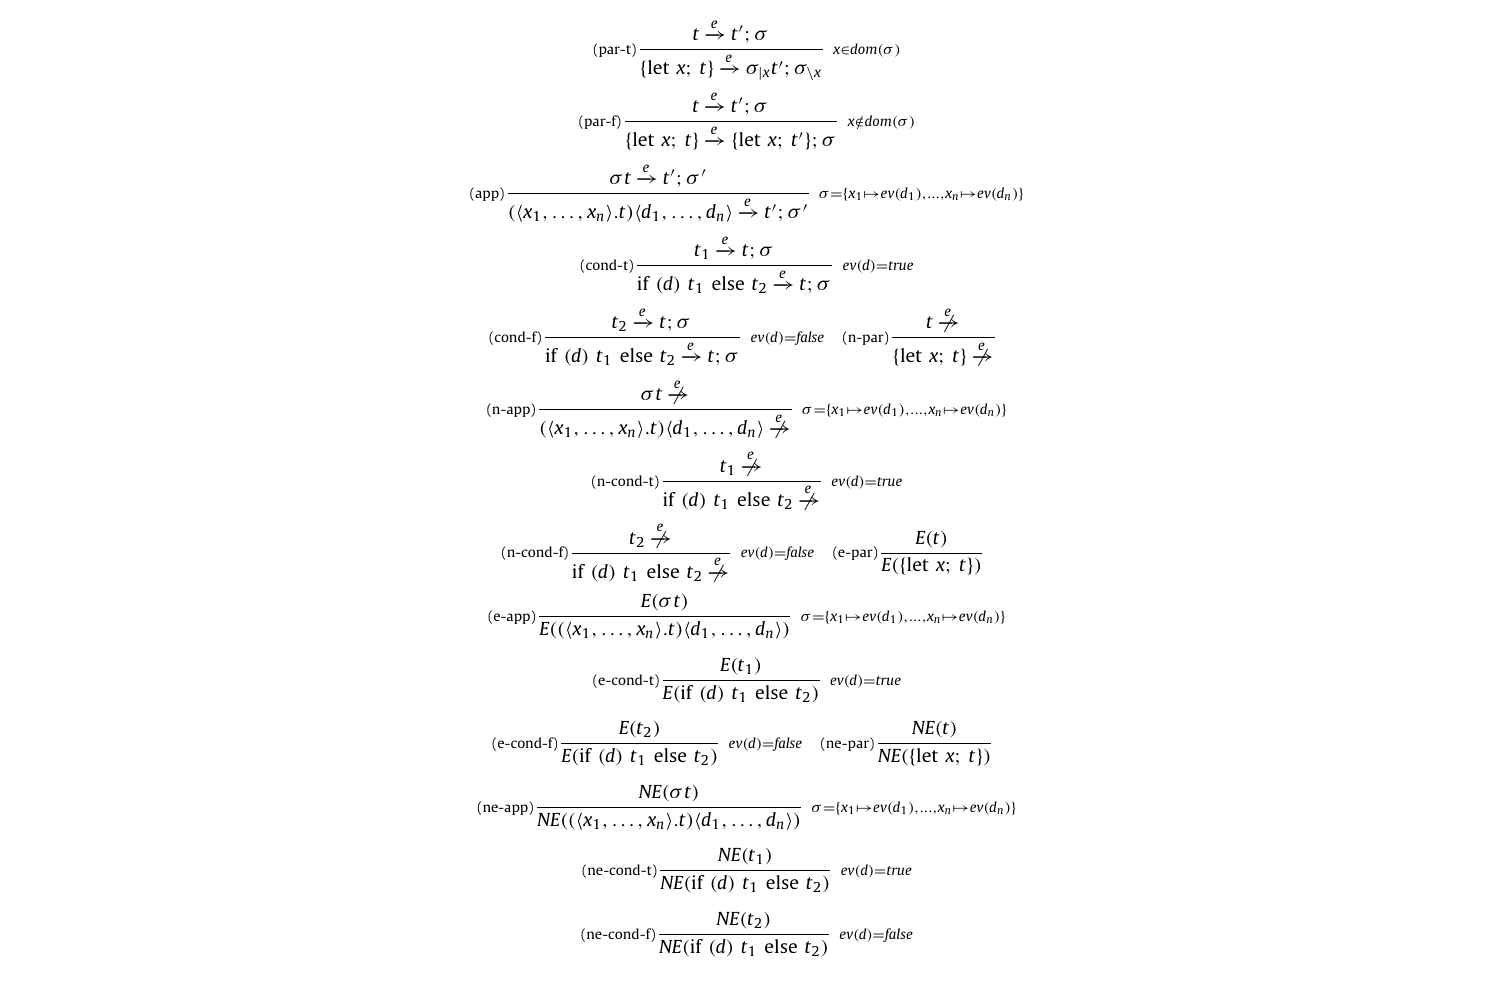
\includegraphics[keepaspectratio,height=0.85\textheight]{images/semantics}
  \end{center}
\end{frame}

%%%%%%%%%%%%%%%%%%%%%%%%%%%%%%%%%%%%%%%%%%%%%%%%%%

\section{Specification of safe hash sets}

\begin{frame}[fragile]{Specification of safe hash sets}
  \begin{block}{Declaration of event types}
    \begin{lstlisting}[basicstyle=\ttfamily\scriptsize]
new_hash(hash_id) matches
  {event:'func_post', name:'HashSet', resultId:hash_id};
not_new_hash not matches new_hash(_);

add(hash_id,elem_id) matches
  {event:'func_post', targetId:hash_id, name:'add',
   argIds:[elem_id], res:true};
not_add(hash_id) not matches add(hash_id,_);

remove(hash_id,elem_id) matches
  {event:'func_post', targetId:hash_id, name:'remove',
   argIds:[elem_id], res:true};

modify(targ_id) matches add(targ_id,_) | remove(targ_id,_);

not_modify_remove(hash_id,elem_id) not matches
  modify(elem_id) | remove(hash_id,elem_id);
op(hash_id,elem_id) matches
  {targetId:hash_id} | {targetId:elem_id};      
    \end{lstlisting}
  \end{block}
\end{frame}

%%%%%%%%%%%%%%%%%%%%%%%%%%%%%%%%%%%%%%%%%%%%%%%%%%

\begin{frame}[fragile]{Specification of safe hash sets}
  \begin{block}{Whole specification}
    \begin{lstlisting}[basicstyle=\ttfamily\scriptsize]
Main = not_new_hash*
  {let hash_id;new_hash(hash_id)(SafeHashSet<hash_id> /\ Main)}?;

SafeHashSet<hash_id> = not_add(hash_id)*
  {let elem_id;add(hash_id,elem_id)(SafeHashElem<hash_id,elem_id> /\ SafeHashSet<hash_id>)}?;

SafeHashElem<hash_id,elem_id> = not_modify_remove(hash_id,elem_id)* (remove(hash_id,elem_id) all)?;
    \end{lstlisting}
  \end{block}
\end{frame}

%%%%%%%%%%%%%%%%%%%%%%%%%%%%%%%%%%%%%%%%%%%%%%%%%%

\begin{frame}[fragile]{Monitor at work}
  \begin{block}{Events}
    \begin{itemize}
    \item  new hash set with id 5
    \item  new hash set with id 9
    \item insertion of set with id 9 into set with id 5  
    \end{itemize}
  \end{block}

  \begin{block}{Reached state}
    \begin{lstlisting}[basicstyle=\ttfamily\footnotesize]

(SafeHashElem<5,9> /\ SafeHashSet<5>) /\ (SafeHashSet<9> /\ Main);

    \end{lstlisting}
  \end{block}
\end{frame}

%%%%%%%%%%%%%%%%%%%%%%%%%%%%%%%%%%%%%%%%%%%%%%%%%%

\begin{frame}[fragile]{Monitor at work}
  \begin{block}{Preliminary experiments}
    \begin{itemize}
    \item  aim: validation of the specification 
    \item  on event traces that simulate the  execution of simple Java programs
    \end{itemize}
  \end{block}
\end{frame}

%%%%%%%%%%%%%%%%%%%%%%%%%%%%%%%%%%%%%%%%%%%%%%%%%%

\begin{frame}[fragile]{Monitor at work}
  \begin{block}{Preliminary experiments: example}
    \begin{lstlisting}[basicstyle=\ttfamily\footnotesize]
var sset = new HashSet<Set<Integer>>();
var s1 = new HashSet<Integer>();
var s2 = new HashSet<Integer>();
s1.add(1);
s2.add(2);
sset.add(s1);
s1.contains(1);
s1.add(1);
sset.add(s2);
sset.remove(s1);
//s2.remove(2);
s1.remove(1);
s2.remove(1);
sset.remove(s2);
s1.add(1);
s2.add(2);
    \end{lstlisting}
  \end{block}
\end{frame}

%%%%%%%%%%%%%%%%%%%%%%%%%%%%%%%%%%%%%%%%%%%%%%%%%%

\begin{frame}[fragile]{Generalization of the specification}
  \begin{block}{Extension to other methods and classes}
    \begin{lstlisting}[basicstyle=\ttfamily\footnotesize]
new_hash(hash_id) matches {event:'func_post', name:'HashSet' | 'HashMap', resultId:hash_id};

add(hash_id,elem_id) matches // addition to a set
  {event:'func_post', targetId:hash_id, name:'add',  
   argIds:[elem_id], res:true}
 |   // addition to a map  
  {event:'func_post', targetId:hash_id, name:'put',  
   argIds:[elem_id,_]};

clear(hash_id) matches  {event:'func_pre', targetId:hash_id, name:'clear'}; 
    \end{lstlisting}

  \end{block}
  \alert{Remark:}
  \begin{itemize}
  \item with \lstinline{put} and \lstinline{clear} is not possible to monitor modification accurately
  \item false positives are possible
  \item the same specification can be used also for Kotlin and Scala
  \end{itemize}
  \end{frame}

%%%%%%%%%%%%%%%%%%%%%%%%%%%%%%%%%%%%%%%%%%%%%%%%%%

\begin{frame}[fragile]{Assessment of the approach}
  \begin{block}{Experiments with real Java applications}
    \begin{itemize}
    \item scalability
    \item ability to detect bugs
    \end{itemize}
  \end{block}
  \end{frame}

%%%%%%%%%%%%%%%%%%%%%%%%%%%%%%%%%%%%%%%%%%%%%%%%%%

\begin{frame}{Q\&A time}
\vspace*{16ex}
  \begin{center}
  \LARGE Thank you!
\end{center}
\end{frame}

\end{document}
